\section{Bayesian inference of species tree}

%%%%%%%%%%%%%%%%%%%%%%%%%%%%%%%%%%%%%%%%%%%%%%%%%%%%%%%%%%
\subsection{Species \& gene trees}

\begin{frame}\frametitle{Species tree}
	\begin{itemize}
		\item Species tree --- the phylogeny representing the relationships among a group of species
		\begin{figure}[h!]
 			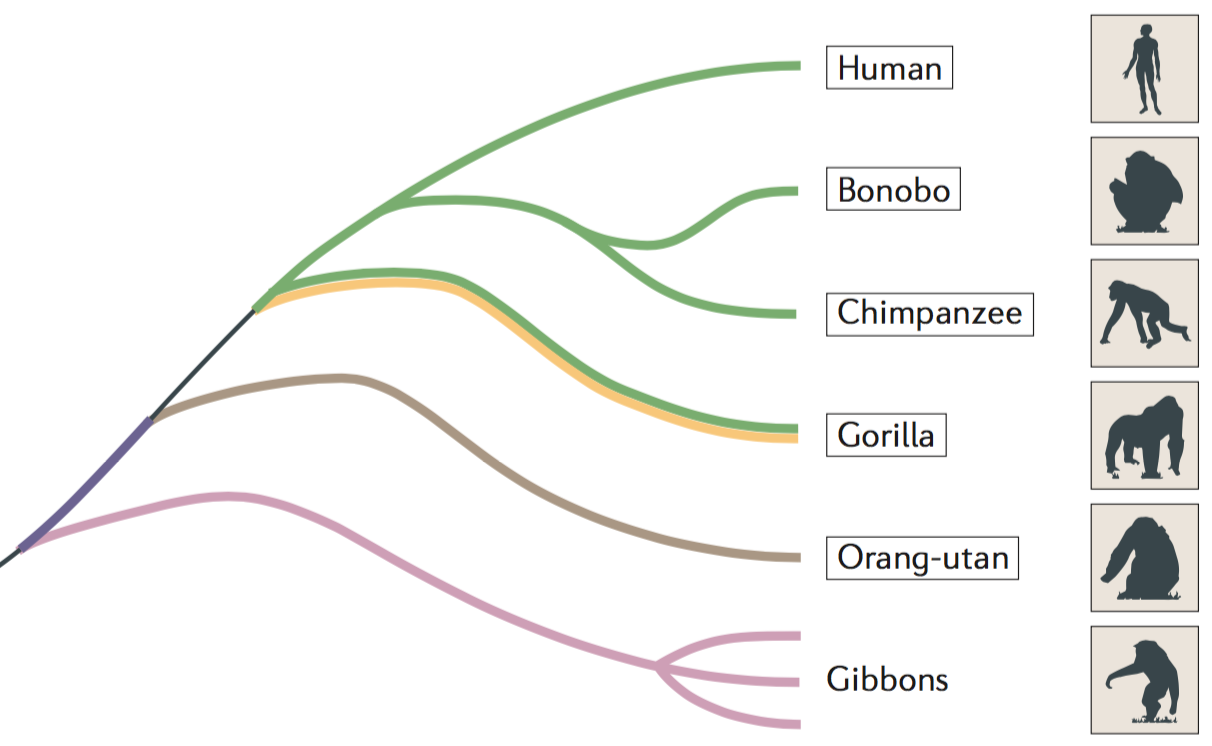
\includegraphics[height=4cm]{figures/primateSpeciesTree}
			\figureCaption{\cite{Rogers:2014ka}}{}
		\end{figure}
		\item Gene tree --- the phylogeny for sequences at a particular gene locus from those species
	\end{itemize}
\end{frame}

\begin{frame}\frametitle{Gene tree discordance}
	\begin{itemize}
		\item Incomplete lineage sorting
	\end{itemize}
	\begin{figure}[h!]
 		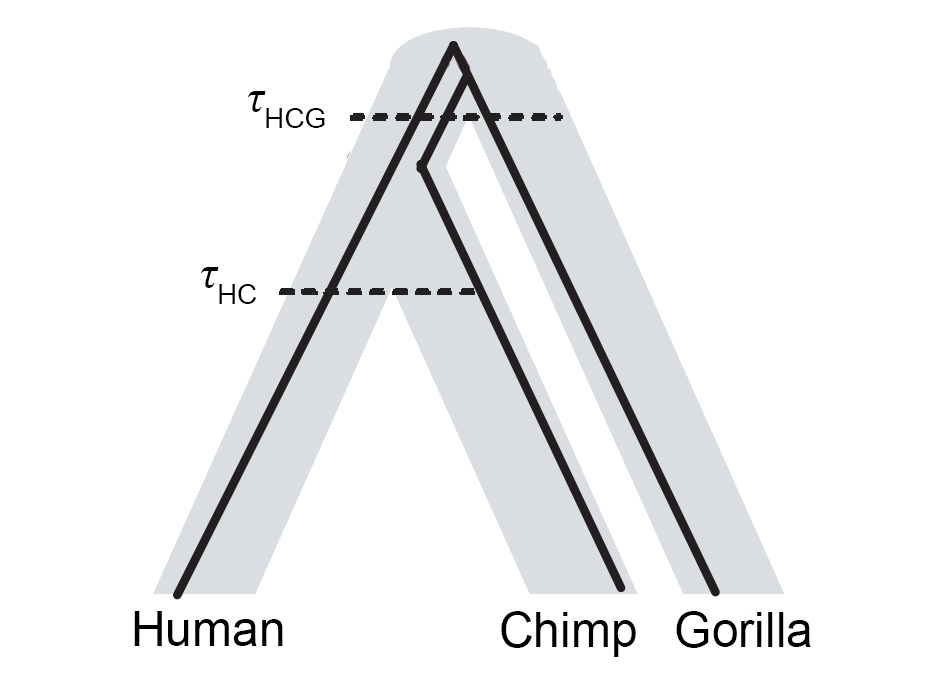
\includegraphics[height=4cm]{figures/incompleteLineageSorting}
		\figureCaption{\cite{Patterson:2006cm}}{}
	\end{figure}
\end{frame}

\begin{frame}\frametitle{Gene tree discordance}
	\begin{itemize}
		\item Horizontal gene transfer
		\item Gene duplication and loss
		\begin{figure}[h!]
 			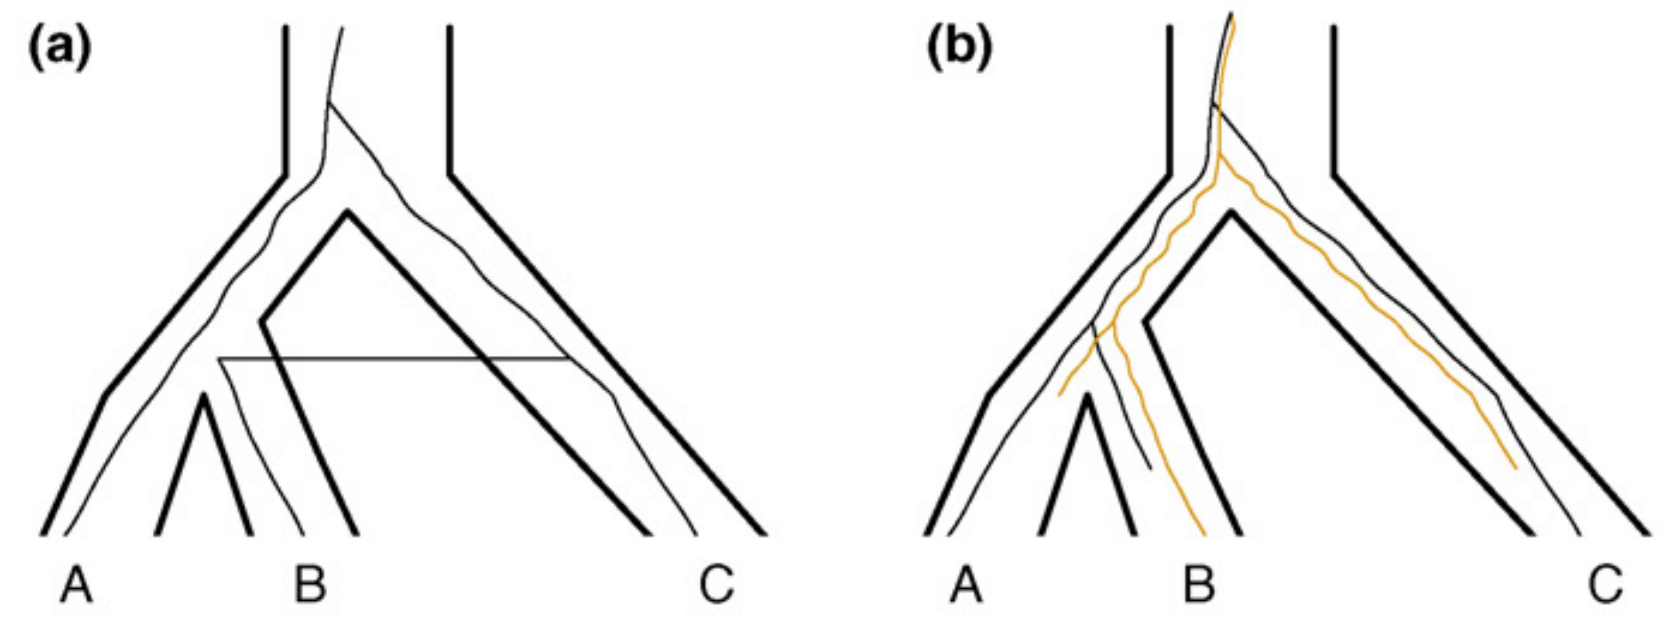
\includegraphics[height=3.5cm]{figures/HGTandDuplicationLoss}
 			\figureCaption{\cite{Degnan:2009hr}}{}
		\end{figure}
	\end{itemize}
\end{frame}

\begin{frame}\frametitle{Gene tree discordance}
	\begin{itemize}
		\item Hybridization
		\begin{figure}[h!]
 			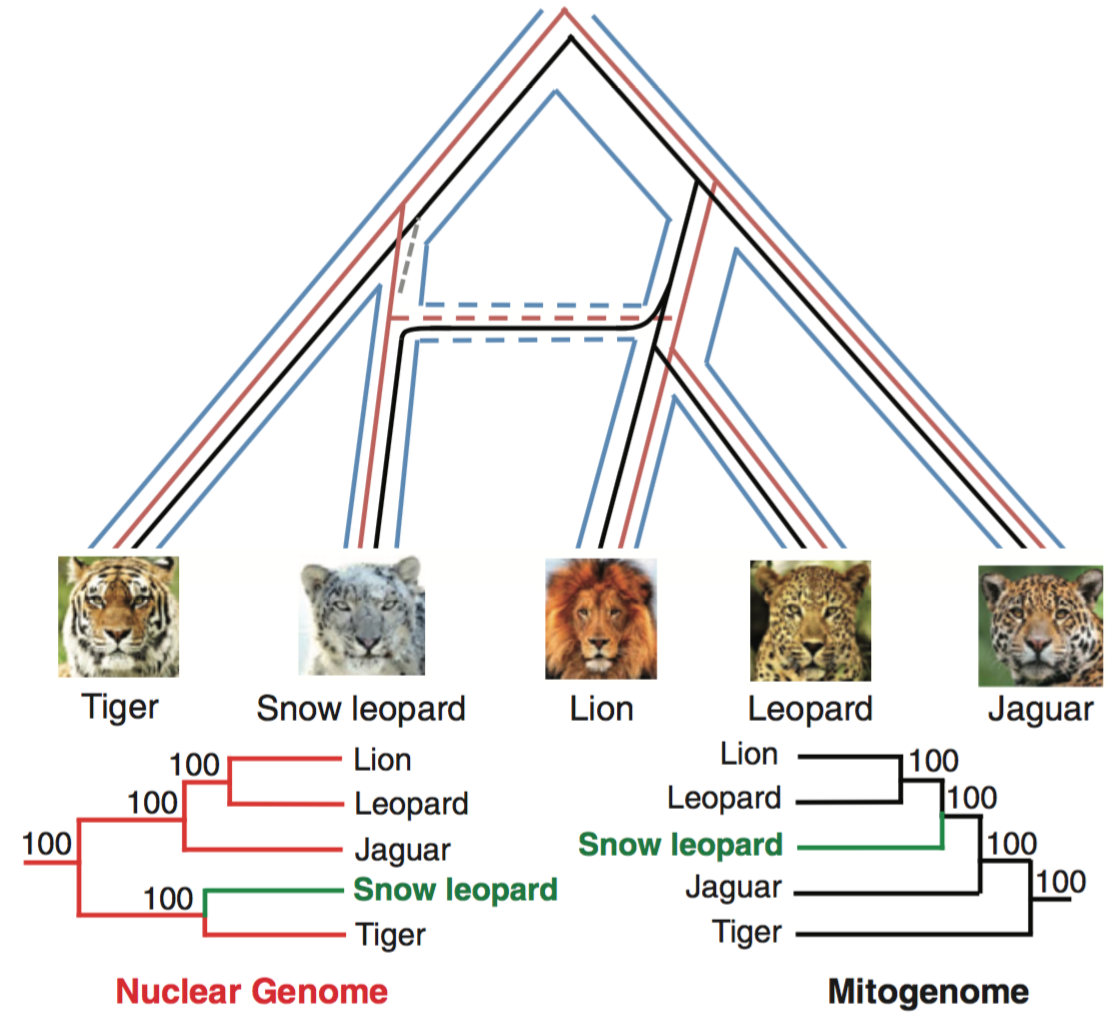
\includegraphics[height=6cm]{figures/hybridization}
 			\figureCaption{\cite{Li:2016ko}}{}
		\end{figure}
	\end{itemize}
\end{frame}

%%%%%%%%%%%%%%%%%%%%%%%%%%%%%%%%%%%%%%%%%%%%%%%%%%%%%%%%%%
\subsection{*BEAST}

\begin{frame}\frametitle{Species tree inference and *BEAST}
	\begin{itemize}
		\item A Bayesian method to infer species tree from multilocus sequence data \cite{Heled:2010ia}
		\item *BEAST, a functionality of BEAST2
	\end{itemize}
	\begin{columns}
	\column{4.6cm}
	\begin{itemize}
		\item Gene trees are embedded in the species tree under the multispecies coalescent model \cite{Rannala:2003vt}
		\begin{itemize}
			\item incomplete lineage sorting
		\end{itemize}
		\item Gene trees are independent among loci
	\end{itemize}
	\column{4.7cm}
    \begin{figure}[h!]
    	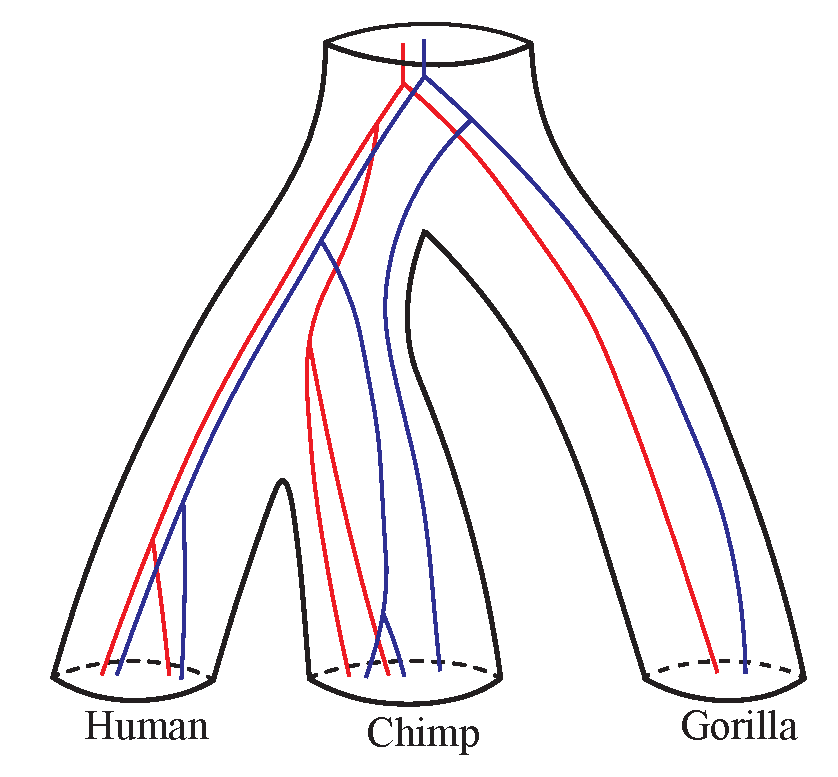
\includegraphics[width=1.0\textwidth]{figures/geneTreesInSpeciesTree}
  	\end{figure}
	\end{columns}
\end{frame}

%\begin{frame}\frametitle{Species tree inference and *BEAST}
%	\begin{itemize}
%		\item TODO: draw a graphical model representation
%	\end{itemize}
%\end{frame}

%%%%%%%%%%%%%%%%%%%%%%%%%%%%%%%%%%%%%%%%%%%%%%%%%%%%%%%%%%
\subsection{Species tree prior}

\begin{frame}\frametitle{Species tree prior}
	\begin{itemize}
		\item The prior for species tree $S$ has two parts:
		\[ P(S) = P(S_T)P(N) \]
		\begin{itemize}
			\item $S_T$ --- species time tree 
			\item $N$ --- population size functions 
		\end{itemize}
		\item $P(S_T)$ --- typically a Yule (pure-birth) or birth-death prior
		\begin{itemize}
			\item we can assign a hyperprior for the speciation (birth) rate (and extinction (death) rate, if birth-death) 
		\end{itemize}
		\item $P(N)$ --- constant or continuous-linear
	\end{itemize}
\end{frame}

\begin{frame}\frametitle{Species tree prior}
	\begin{itemize}
		\item Constant population sizes
		\begin{figure}[h!]
 			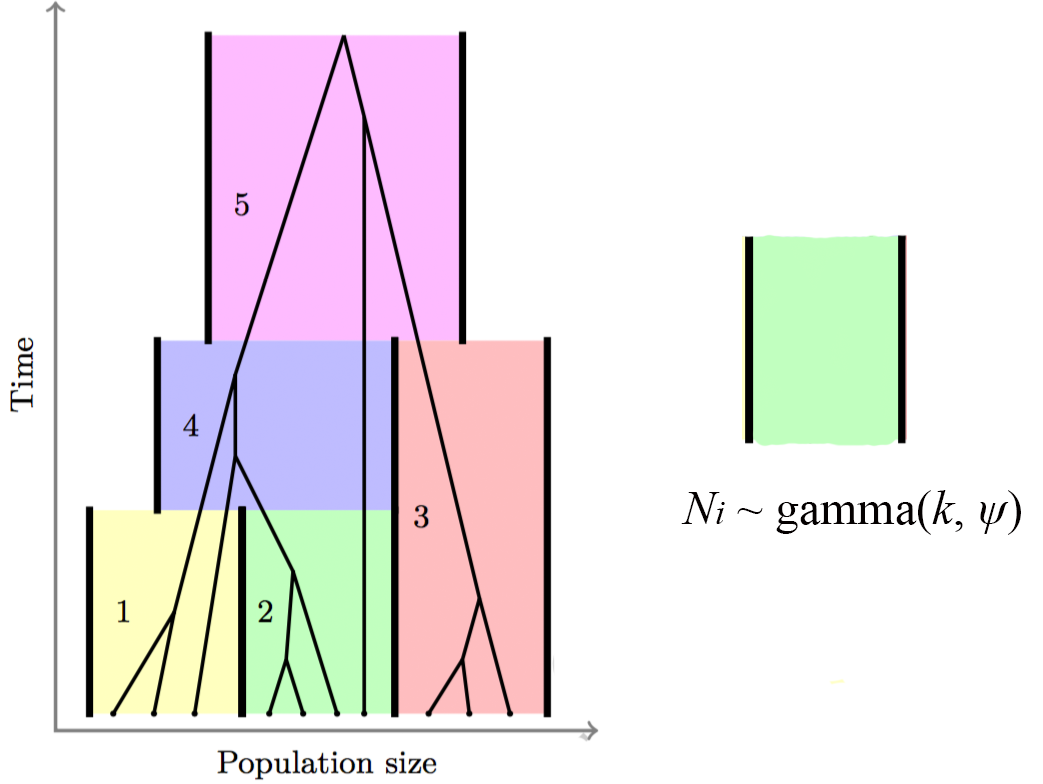
\includegraphics[height=5cm]{figures/popFunctionConstant}
 			\figureCaption{\cite{Drummond:2015tz}}{}
		\end{figure}
	\end{itemize}
\end{frame}

\begin{frame}\frametitle{Species tree prior}
	\begin{itemize}
		\item Continuous-linear population sizes
		\begin{figure}[h!]
 			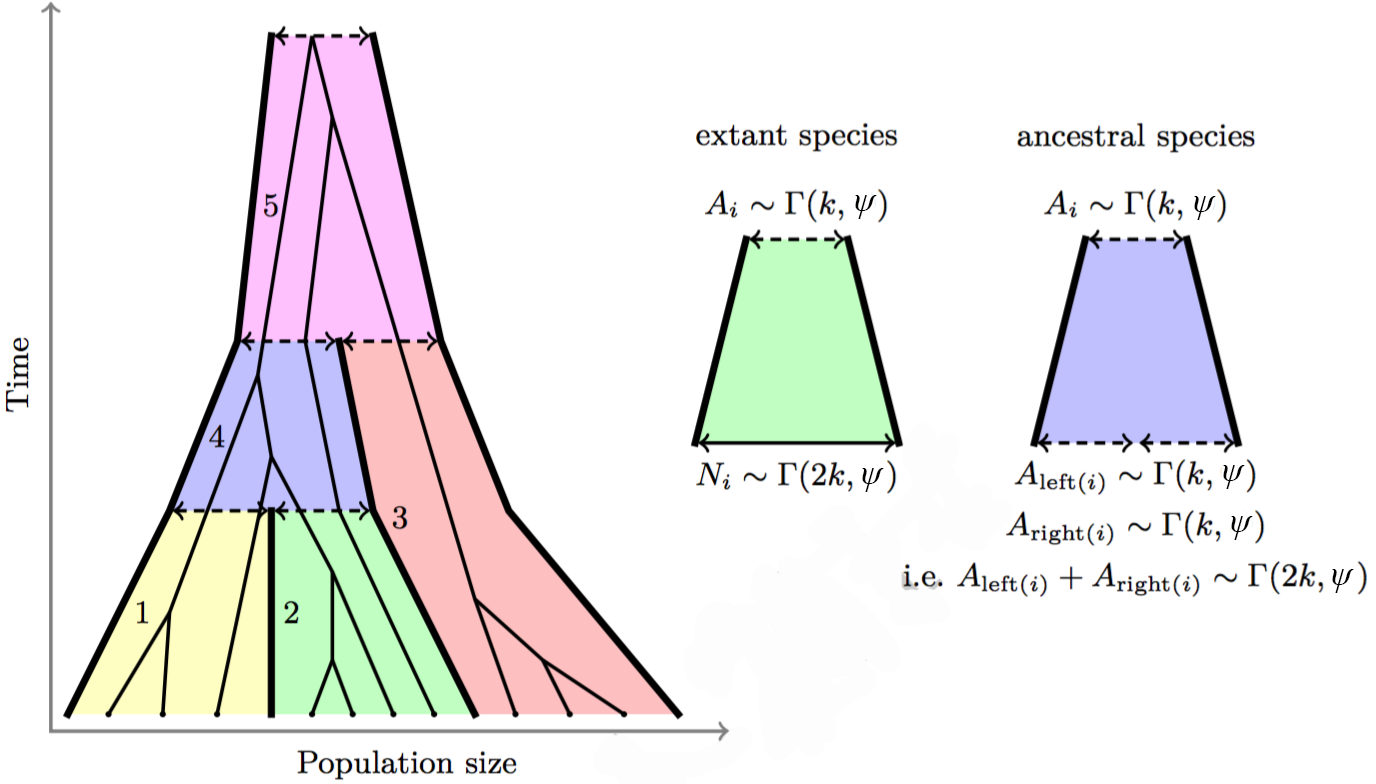
\includegraphics[height=5.3cm]{figures/popFunctionLinear}
 			\figureCaption{\cite{Drummond:2015tz}}{}
		\end{figure}
	\end{itemize}
\end{frame}

\begin{frame}\frametitle{Species tree prior}
	\begin{itemize}
		\item In *BEAST, the prior type for $N$ is fixed to gamma
		\item The gamma shape parameter $k$ is fixed to 2, but we can assign a hyperprior for $\psi$, the scale parameter of the gamma
		\item (This $\psi$ parameter is called "population mean" in Beauti, but the prior mean is actually $2\psi$ when the population sizes are constant) 
	\end{itemize}
\end{frame}

%%%%%%%%%%%%%%%%%%%%%%%%%%%%%%%%%%%%%%%%%%%%%%%%%%%%%%%%%%
\subsection{Multispecies coalescent}

\begin{frame}\frametitle{Multispecies coalescent model}
	\begin{itemize}
		\item The prior for gene tree $g$, given species tree $S$
	\end{itemize}
	\begin{figure}[h!]
 		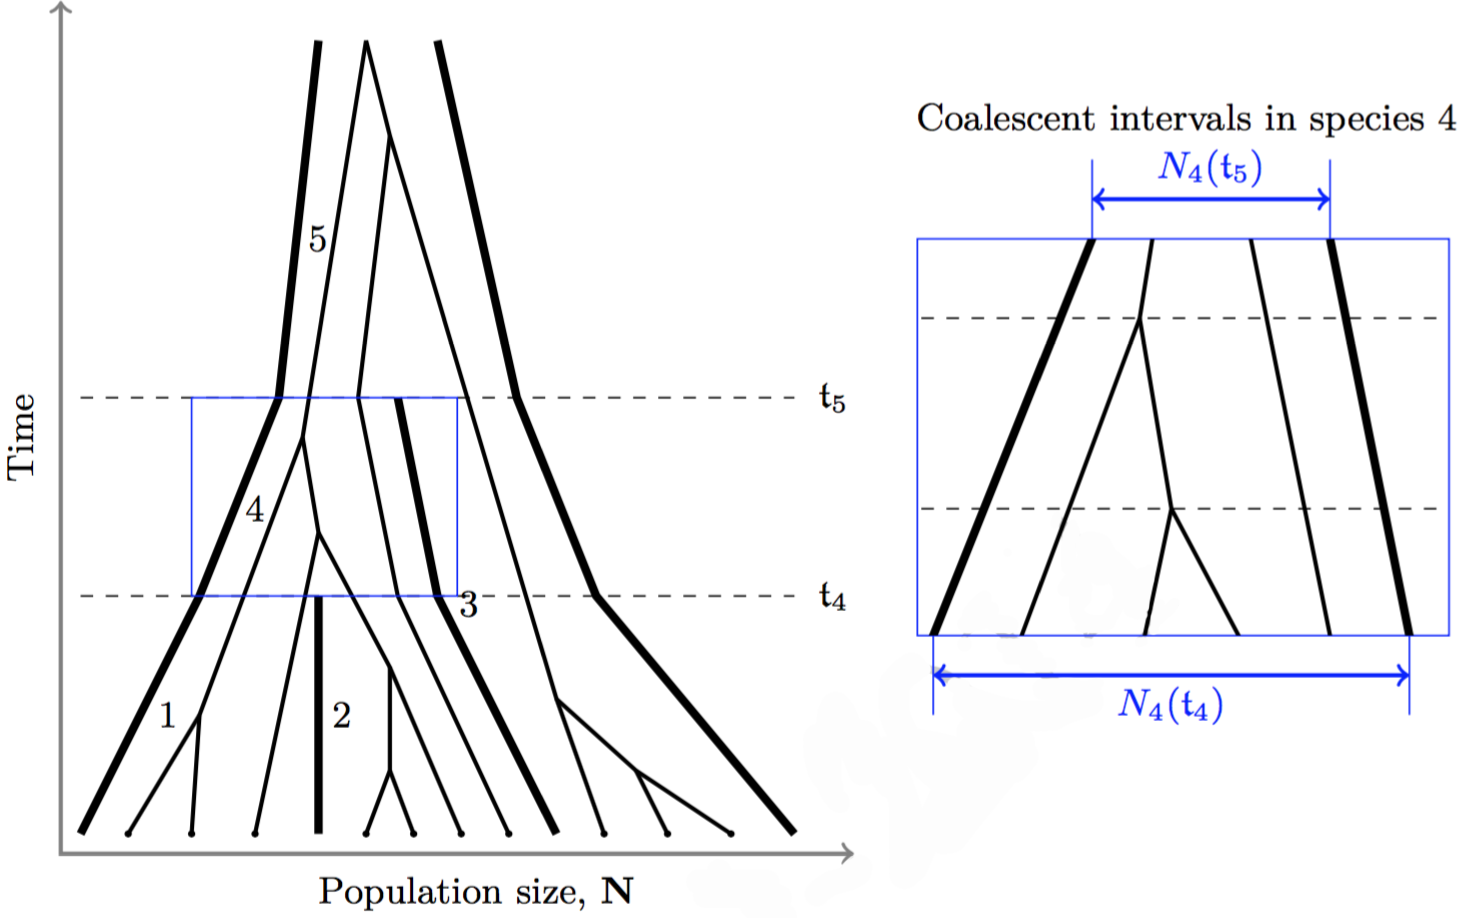
\includegraphics[height=5.5cm]{figures/mscOverview}
 		\figureCaption{\cite{Drummond:2015tz}}{}
	\end{figure}
\end{frame}

\begin{frame}\frametitle{Multispecies coalescent model}
	\begin{itemize}
		\item The prob. distribution of gene time tree $g$ given species tree $S$, is:		
		\[ P(g|S) = \prod_{j=1}^{2s-1} P(L_j(g)|N_j(t)) \]
	\end{itemize}
	\begin{columns}
	\column{5.4cm}
		\begin{itemize}
			\item $s$ --- number of extant species ($2s-1$ branches totally)
			\item $N_j(t)$ --- population size function (linear)
			\item $L_j(g)$ --- coalescent intervals for genealogy $g$ that are contained in the $j$'th branch of species tree $S$
		\end{itemize}
	\column{4cm}
    \begin{figure}[h!]
    	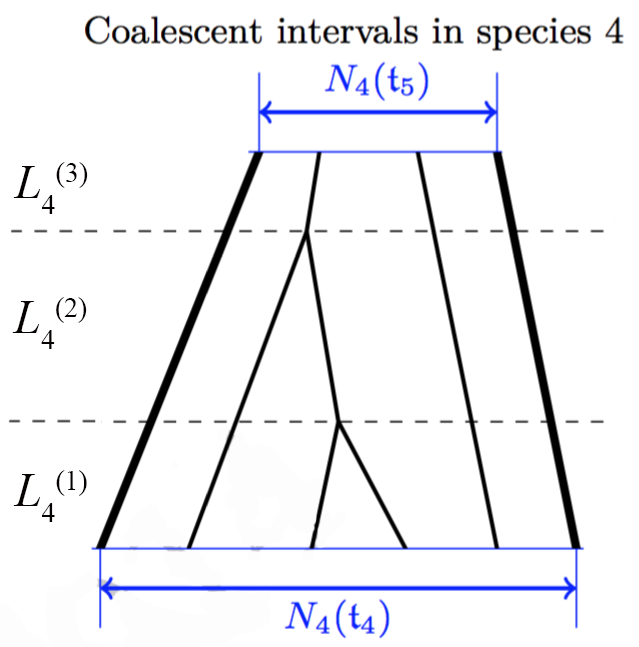
\includegraphics[width=1.0\textwidth]{figures/mscPopulation4}
  	\end{figure}
	\end{columns}
\end{frame}

%%%%%%%%%%%%%%%%%%%%%%%%%%%%%%%%%%%%%%%%%%%%%%%%%%%%%%%%%%
\subsection{Molecular clock model}

\begin{frame}\frametitle{Molecular clock model}
	\begin{itemize}
		\item $P(c)$ --- prior for the molecular clock model of genealogy $g$
		\begin{itemize} 
			\item strict clock --- typically fix to 1.0 for the first locus, and infer the relative clock rates for the rest loci
			\item relaxed clock
		\end{itemize}
	\end{itemize}
	\begin{itemize}
		\item $P(\theta)$ --- prior for the substitution model parameters
		\item e.g. HKY85,
		\begin{itemize} 
			\item Prior for transition/transversion rate ratio ($\kappa$), e.g. gamma(2,1)
  			\item Prior for base frequencies ($\pi_T, \pi_C, \pi_A, \pi_G$), e.g. Dirichlet(1,1,1,1)
		\end{itemize}
	\end{itemize}
\end{frame}

%%%%%%%%%%%%%%%%%%%%%%%%%%%%%%%%%%%%%%%%%%%%%%%%%%%%%%%%%%
\subsection{Felsenstein likelihood}

\begin{frame}\frametitle{Felsenstein likelihood}
	\begin{itemize}
		\item The probability (likelihood) of data $d_i$ (alignment at locus $i$), given the gene time tree $g_i$, molecular clock $c_i$, and substitution model $\theta_i$, is:
		\[ P(d_i|g_i,c_i,\theta_i) \]
	\end{itemize}
\end{frame}

%%%%%%%%%%%%%%%%%%%%%%%%%%%%%%%%%%%%%%%%%%%%%%%%%%%%%%%%%%
\subsection{Posterior distribution}

\begin{frame}\frametitle{Priors and likelihood}
	\begin{itemize}
		\item $P(S)$ --- prior for species tree
		\vskip 0.4cm 
		\item $P(g_i|S)$ --- prior for gene tree $i$ (multispecies coalescent)
		\vskip 0.4cm
		\item $P(c_i)$ --- prior for clock rate of locus $i$
		\vskip 0.4cm
		\item $P(\theta_i)$ --- prior for substitution parameters of locus $i$
		\vskip 0.4cm
		\item $P(d_i|g_i,c_i,\theta_i)$ --- likelihood of data at locus $i$
	\end{itemize}
\end{frame}

\begin{frame}\frametitle{Posterior}
	\begin{itemize}
		\item The posterior distribution of the species tree $S$ and other paremeters given data $D$ is:
		\[ P(S, \mathbf{g, c}, \Theta|D) \propto P(S) \prod_{i=1}^n P(g_i|S) P(c_i) P(\theta_i) P(d_i|g_i,c_i,\theta_i) \]
		\item The data $D = \{d_1, d_2, \dots, d_n\}$ is composed of $n$ alignments, one per locus.
	\end{itemize}
\end{frame}

%%%%%%%%%%%%%%%%%%%%%%%%%%%%%%%%%%%%%%%%%%%%%%%%%%%%%%%%%%
\subsection{starBEAST2}

\begin{frame}\frametitle{Integrating out population sizes}
	\begin{itemize}
		\item Assume constant population sizes
		\item Assign i.i.d inverse-gamma($\alpha$, $\beta$) prior for $N_j$ 
		\begin{itemize}
			\item mean = $\beta / (\alpha -1)$
		\end{itemize}
		\item The population sizes $N$ can be integrated out from $P(g|S)$ \cite{Jones:2015jf}
		\vskip 0.4cm
		\item Specify $\alpha$ and $\beta$ in the invgamma prior (instead of $\psi$ in the gamma prior)
	\end{itemize}
\end{frame}

\begin{frame}\frametitle{starBEAST2}
	\begin{itemize}
		\item A more efficient implementation and an upgrade of *BEAST
		\begin{itemize}
			\item Population sizes integrated out \cite{Jones:2015jf}
			\item Relaxed molecular clock per species tree branch (instead of per gene tree branch)
			\item More efficient MCMC proposals for the species tree and gene trees (coordinated operators) \cite{Jones:2015jf, Rannala:2015wk}
		\end{itemize}
		\item Available at \url{github.com/genomescale/starbeast2}, will be released soon (as a BEAST2 add-on)
	\end{itemize}
\end{frame}

